\chapter{Theoretische Fundierung von KI-gestützten Chatbots im Coaching} \label{chap:2}
Künstliche Intelligenz (KI) ist ein multidisziplinäres Forschungsgebiet, mit Fokus auf der Entwicklung intelligenter Maschinen, die in der Lage sind, Aufgaben zu bewältigen, die normalerweise menschliche Intelligenz erfordern \citep{Sangeetha2023Introduction}. Dazu gehören Aufgaben wie Problemlösung, Entscheidungsfindung, Lernen und das Verstehen natürlicher Sprache. Die KI verfolgt das Ziel, Systeme zu schaffen, die menschliche kognitive Fähigkeiten nachahmen oder replizieren können. Maschinelles Lernen als Teilgebiet der  künstlichen Intelligenz betrachtet die Entwicklung von Algorithmen und statistischen Modellen. Diese befähigen Maschinen auf der Grundlage von Daten zu Lernen und Entscheidungen zu treffen, sowie Vorhersagen zu machen. Deep Leraning meint in diesem Zusammenhang die Anwendung vielschichtiger neuronaler Netze, um aus den unterschiedlichen Abstraktionsebenen der Daten zu lernen.


Ein KI-basiertes Anwendungssystem unterstützt den Anwender dabei, fachliche Aufgaben auf der Grundlage von KI, sowie des Einsatzes von Hardware, Software, sowie möglicherweise logischen Elementen \citep{grum2022construction}. Der Nutzer verwendet die Ergebnisse des KI-basierten Systems und liefert gleichzeitig Daten, die wiederum von dem System genutzt werden.
Chatbots sind KI-basierte Sprachmodelle. Ihre Anwendung und Funktionsweise wird im Folgenden erläutert.

\section{Funktionsweisen von Sprachmodellen}
Unter Natural Language Processing (NLP) versteht man einen Prozess, bei dem Computer menschliche Sprache verstehen, interpretieren und generieren \citep{Sangeetha2023Introduction}. Dies beinhaltet Aufgaben wie Spracherkennung, Sentiment-Analyse, Sprachübersetzung und die Beantwortung von Fragen. 

Large Language Models (LLMs) stellen ein Teilbereich des NLP und damit der künstlichen Intelligenz \citep{Raiaan2024A}. Dies sind Modelle zur Verarbeitung und Generierung natürlicher Sprache. Der Fokus liegt auf dem Training großer Mengen an Textdaten mit dem Ziel, die Bedeutung von Zusammenhängen zu erlernen. Ausgereifte LLMs verfügen über eine Vielzahl von Fähigkeiten, darunter die Generierung, Informationsgewinnung und Zusammenfassung von Texten, sowie die Beantwortung von Fragen, Übersetzung von Sprache, Unterstützung bei Dialogen und Konversationen und das Erzeugen von kontextbezogenen Antworten. Statistische Muster werden genutzt, um Informationen für Vorhersagen nutzbar zu machen. Das bedeutet, getätigte Eingaben werden datenbasiert verarbeitet. Es besteht die Möglichkeit, komplexe sprachliche Strukturen zu erkennen und diese nachzubilden. 

\subsection{Technische Grundlagen von LLMs}
LLMs basieren überwiegend auf der Transformer-Architektur \citep{vaswani2017attention}. Sie zeichnen sich durch eine hohe Skalierbarkeit, parallele und effiziente Verarbeitung langer Texte, sowie einer guten Erfassung von Kontextinformationen aus. 

Zur Verarbeitung der Texte werden diese in einzelne Tokens zerlegt werden \citep{grum2022construction, vaswani2017attention}. Diese sind zum Beispiel Wörter oder einzelne Wortbestandteile, sowie Zeichen oder Symbole. Dann erfolgt die Umwandlung der natürlichen Sprache in maschinenlesbare Einheiten. Diese numerische Darstellung der Tokens als Vektoren wird als Embedding bezeichnet und ermöglicht eine mathematische Verarbeitung der Sprache. Wörter, die eine ähnliche Bedeutung haben liegen im Vektorraum nahe beieinander. Das Konzept des Positional Encoding sorgt in diesem Zusammenhang dafür, ein Verständnis von Satzstruktur und Wortfolge beizubehalten. Besonderes relevante Informationen werden für die gewollte Ausgabe gewichtet. Es werden drei Arten der Attention unterschieden. Self-Attention betrachtet die Beziehungen innerhalb derselben Eingabesequenz, Cross-Attention stellt eine Verknüpfung von Encoder- und Decoder-Informationen bereit und die Full Attention schließlich eine vollständige Berücksichtigung aller Tokens. Der Encoder verarbeitet die Eingabesequenz und wandelt sie in eine mathematische Repräsentation um, die Informationen über die Bedeutung der einzelnen Tokens und ihre Beziehungen zueinander enthält. Durch Decoding wird schließlich eine Ausgabesequenz generiert, welche auf Grundlage der bisher verwendeten Tokens, schrittweise das nächste Token voraussagt. Ausgewählt werden je Folgetokens mit höchster Wahrscheinlichkeit.

Das Training von LLMs basiert auf großen Mengen an Textdaten \citep{Raiaan2024A}. Beim Pre-Training findet ein Lernen allgemeiner Sprachmuster und Wissensrepräsentationen statt. Typische Trainingsdaten stammen aus Webseiten, Büchern oder wissenschaftlichen Texten. Die Erkenntnisse werden anschließend zur Anpassung an spezifische Aufgaben durch Finetuning genutzt. Das vortrainierte Modell wird an spezifische Aufgaben angepasst. Dafür werden kleinere und kontextrelevante Datensätze verwendet. Für den Trainingsprozess ist eine qualitative Datenaufbereitung von Bedeutung. Dies beinhaltet die Entfernung fehlerhafter oder irrelevanter, sowie doppelter Daten und die Exklusion personenbezogener Informationen. Normalisierung ermöglicht anschließend die Stabilisierung des Trainingsprozesses und ermöglicht das Lernen komplexer Muster. Das Verfahren zeichnet sich durch hohen Rechenaufwand und Speicherbedarf, sowie lange Trainingszeiten aus.

\subsection{Neuronale Netzwerke und neuronale Modelle}
Künstliche neuronale Netzwerke (Artificial Neural Networks, ANN) sind rechnergestützte Modelle \citep{grum2022construction,nielsen2015neural,kinnebrock2018neuronale}. Sie orientieren sich an der Struktur und Funktionsweise biologischer Nervensysteme. Diese bestehen aus miteinander verbundenen künstlichen Neuronen, die Informationen verarbeiten und durch Anpassung ihrer Verbindungsgewichte Muster und Zusammenhänge aus Daten erlernen können. 
Neuronale Modellierung basiert auf der mathematischen oder computergestützten Darstellung von Systemen, die sich an der Funktionsweise von biologischen Nervenzellen orientieren. Auf diese Weise werden Prinzipien der Neurowissenschaft, Mathematik und Informatik vereint, um ein Verständnis darüber zu schaffen, wie ein System auf Basis von Neuronen funktioniert und wie diese miteinander interagieren. Ziel des Konzeptes neuronaler Modellierung ist es, komplexe Verhaltensweisen zu erklären.  
Neuronale Netzwerke lernen basierend auf Trainingsdaten, um Vorhersagen zu treffen oder spezifische Aufgaben zu lösen. Aufgrund ihrer Fähigkeit, komplexe und nicht-lineare Zusammenhänge zu modellieren, bilden neuronale Netzwerke die Grundlage moderner Verfahren des Deep Learnings. Ein Modell stellt eine vereinfachte und zweckorientierte Abbildung eines realen oder künstlichen Systems dar. Es beschreibt ausgewählte Elemente, deren Beziehungen sowie relevante Eigenschaften eines Systems, um dessen Struktur und Verhalten verständlich zu machen. Modelle werden verwendet, um Systeme zu beschreiben, analysieren, simulieren, entwerfen oder zu bewerten. Sie werden entsprechend ihres jeweiligen Anwendungszwecks erstellt. 

\subsubsection{Biologischer Hintergrund künstliche neuronaler Netzwerke}
Künstliche neuronale Netze basieren auf der Funktionsweise des menschlichen Nervensystems basieren \citep{grum2022construction,lammel2012kunstliche}. Ziel ist es, das Prinzip eines biologischen Systems auf ein technisches System zu übertragen. Das Nervensystem beinhaltet das Zentralnervensystem (ZNS), sowie sensorischen und motorischen Systemen. Diese bestehen aus Nervenzellen, den sogenannten Neuronen, welche als Signalträger fungieren. Gliazellen dienen dabei als unterstützende Struktur und haben die Aufgabe, der strukturellen Stabilisierung neuronaler Netzwerke. Sie versorgen Neuronen mit Nährstoffen und unterstützen beim Aufbau neuronaler Verbindungen. Die Informationsverarbeitung im Gehirn erfolgt über elektrische Potenzialänderungen und Frequenz von Nervenimpulsen. Die Interaktion der Neuronen, unterscheidet sich zwischen elektrischer und chemischer Signalübertragung.
Aus diesem Grund ist der Aufbau eines Neurons, als Signalverarbeitungseinheit relevant, um zu verstehen, wie diese sich in einem neuronalen Netzwerk zusammenfügen. Neuronen bestehen aus Dendriten, die eingehende, meist chemischer Signale empfangen. Während diese hauptsächlich über kurze Distanzen Signale übertragen, dienen Axone für eine schnelle Signalweiterleitung über längere Distanzen. Sie leiten vor allem elektrische Signale weiter. Synapsen wandeln chemische Signale in elektrische um und ermöglichen die Übertragung und Kommunikation zwischen Neuronen. Die Verarbeitung der Information erfolgt im Zellkörper.

\begin{figure}[h!]
    \centering
    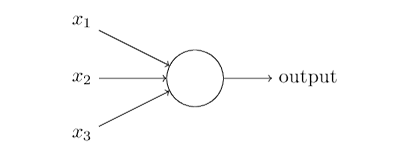
\includegraphics[width=0.5\textwidth]{Bilder/neuron.png}
    \caption{Aufbau eines künstlichen Neurons \citep{nielsen2015neural}}
    \label{fig:neuron}
\end{figure}

\subsubsection{Architektur künstlich neuronaler Netzwerke}
Ein künstliches Neuron stellt eine Funktion dar, die mehrere Eingangssignale in ein Ausgangssignal überführt \citep{nielsen2015neural}. Abbildung \ref{fig:neuron} zeigt diese Transformation anhand eines einfachen Perzeptron. Dieses ist das einfachste Modell eines künstlichen Neurons. Ein Neuron kann ein oder mehrere Eingabewerte (Inputs) $x_1, x_2, \ldots, x_n$ haben, die numerisch dargestellt sind. Sie beinhalten Informationen aus externen Datenquellen oder vorherigen Neuronen. Jedem dieser Werte ist ein Gewicht $w_i$ zugeordnet, welches die Stärke des Einflusses eines Eingangssignals auf die Ausgabe bestimmt. 

Während des Lernprozesses können diese Gewichte angepasst werden, um somit die Ausgabe und Funktionalität des Modells zu verbessern \citep{lammel2012kunstliche}. Es wird zusätzlich ein konstanter Eingabewert integriert. Dieser wird als Bias $b$ bezeichnet. Er erhöht die Flexibilität des Modells. Der Bias und die gewichteten Eingangswerte werden zu einer Gesamtsumme, der sogenannten Aktivierung, zusammengeführt. 

Die gewichtete Summe kann als Zusammenfassung aller verfügbaren Informationen verstanden und durch folgende Gleichung repräsentiert werden \citep{grum2022construction,nielsen2015neural}:
\[a = \sum_{i=1}^{n} w_i x_i + b\]
Dies ist Grundlage der Aktivierungsfunktion, die das Ausgabesignal berechnet. Die Aktivierungsfunktion transformiert die Aktivierung in einen Ausgabewert und führt häufig Nichtlinearitäten ein, wodurch komplexe Zusammenhänge modelliert werden können. Bei einem klassischen Perzeptron erfolgt eine harte Schwellwertentscheidung:
\[
\text{Ausgabe} =
\begin{cases}
1, & \text{wenn die Aktivierung } > 0 \\
0, & \text{wenn die Aktivierung } \le 0
\end{cases}
\]
Das Perzeptron kann somit als einfacher binärer Klassifikator betrachtet werden. Das Ergebnis dieser Funktion bildet dann das Ausgabesignal des Neurons. Auf diese Weise stellt ein künstliches Neuron ein neuronales Modell dar, dass nach biologischen Prinzipien funktioniert. Die Inputs repräsentieren die Dendriten und die Gewichte die Stärke der Synapsen. Die Aktivierungsfunktion entspricht dem Mechanismus, mit dem ein biologisches Neuron entscheidet, ob ein Signal weitergeleitet wird. Ausgabe des künstlichen Neurons ist das Signal, dass schließlich über das Axon an andere Neuronen übertragen wird.

Einzelne Perzeptrone können zu einem Netzwerk zusammengeschlossen werden \citep{nielsen2015neural,kinnebrock2018neuronale}. Die Ausgabe eines Neurons repräsentiert dann die Eingabe für nachfolgende Neuronen. Durch mehrere Schichten der Verarbeitung können auf diese Weise abstrakte Zusammenhänge abgebildet werden. Die Verarbeitung erfolgt schichtweise von links nach rechts. Neuronen in früheren Schichten erkennen einfache Muster und Neuronen in höhere Schichten kombinieren diese Informationen dann zu komplexeren Merkmalen. Auf diese Weise können Entscheidungsprozesse modelliert werden. Moderne Deep-Learning-Modelle verwenden häufig keine einfachen Schwellenfunktionen mehr. Stattdessen werden differenzierbare Aktivierungsfunktionen wie Sigmoid-Funktion oder Tangens-Funktion verwendet. Die Sigmoid-Funktion liefert Werte zwischen 0 und 1. Sie wird häufig für Wahrscheinlichkeitsinterpretationen verwendet. Beim hyperbolischen Tangens (tanh) sind Werte zwischen -1 und +1 um null zentriert.

\subsubsection{Training künstlicher neuronaler Netze}
Der grundlegende Lernprozess eines neuronalen Netzes wird durch die schrittweise Anpassung der Gewichte und Bias-Werte ermöglicht \citep{grum2022construction,lammel2012kunstliche}. Ziel des Trainingsprozesses ist es, die Differenz zwischen den gewünschten, gegebenen Zielwert und dem tatsächlichen Ausgabewert zu minimieren. Dieser Unterschied wird als Vorhersagefehler bezeichnet. Das Lernen erfolgt iterativ, indem der Testdatensatz mehrmals durchläuft. Es endet, wenn ein definiertes Qualitätskriterium erreicht wird oder keine wesentlichen Verbesserungen mehr auftreten. Im ersten Schritt werden die Gewichte der Verbindungen zufällig initialisiert, da noch kein Wissen über bestehende Zusammenhänge existiert. Beim Forward-Pass werden Eingabedaten ausschließlich vorwärts durch das Netz propagiert. Solche Netzwerke werden als Feedforward Neural Networks bezeichnet. Aufgrund mehrerer Schichten spricht man dann häufig von Multilayer Perzeptron (MLP). Der Fehler (Loss) beschreibt, wie stark die Vorhersage von der gewünschten Ausgabe abweicht. Häufig verwendete Fehlerfunktionen sind Mean Squared Error (MSE) oder Cross-Entropy-Loss. MSE berechnet die quadratische Abweichung zwischen Vorhersage und Zielwert. Größere Fehler werden dabei stärker bestraft, weshalb sich dieser vor allem für Regressionsprobleme eignet. Cross-Entropy-Loss wird häufig für Klassifikationsaufgaben verwendet und ermöglicht schnelles, stabiles Lernen. Es wird die Abweichung zwischen vorhergesagten Wahrscheinlichkeiten und tatsächlichen Klassen gemessen. Eine weitere Möglichkeit, wie das Modell trainiert werden kann, ist Backpropagation. Dabei wird zuerst der Fehler berechnet und anschließend von der Ausgabeschicht zur Eingabeschicht zurück propagiert. Es wird ermittelt, welchen Anteil die einzelnen Verbindungen am Gesamtfehler haben, sodass eine individuelle Anpassung der Gewichte die Ausgabe verbessert. Wie stark und in welche Richtung eine Anpassung erfolgen soll, wird durch die Gradienten angegeben. Ziel des Gradientenabstiegs ist es, die Gewichte so zu verändern, dass der Fehler minimiert wird. Die Lernrate $\alpha$ bestimmt die Gewichtsanpassung. Die Wahl der Lernrate beeinflusst maßgeblich den Trainingserfolg. Ist die Lernrate groß, führt dies zu einem schnellen Lernprozess. Jedoch besteht auf diese Weise das Risiko, das Optimum zu überschreiten. Kleinere Lernraten ermöglichen zwar ein stabileres Lernen, haben jedoch eine längere Trainingsdauer. Um Lernschwankungen zu reduzieren und lokale Minima zu überwinden, sowie die Konvergenz zu beschleunigen, kann ein Momentum herangezogen werden. Dieses verleiht dem Lernprozess eine gewisse Trägheit, indem zusätzlich auch frühere Gewichtsanpassungen berücksichtigt werden. Zusätzlich kann zwischen Batch und Online Learning unterschieden werden. Beim Batch Learning erfolgt die Gewichtsanpassung nach Verarbeitung des gesamten Trainingsdatensatzes. Dies führt zu einer stabileren Gradientenberechnung, hat jedoch einen höheren Rechenaufwand. Beim Online Learning werden die Gewichte nach jedem einzelnen Trainingsbeispiel angepasst. Dadurch wird eine schnellere Verarbeitung neuer Informationen ermöglicht. Dies ist besonders geeignet für kontinuierliche Lernprozesse, da das Verfahren robust gegenüber lokalen Minima ist. Um den Lernprozess zu verbessern ist außerdem eine Aufbereitung der Trainingsdaten hilfreich. Dies beinhaltet zum einen die Normalisierung der Daten, um die Trainingsstabilität zu verbessern und zum anderen Generalisierung. Das bedeutet, dass das Modell allgemeine Muster und Zusammenhänge erkennen kann, anstatt auf spezifische Einzelfälle zu betrachten. Das Ergebnis ist dann, eine hohe Leistung auf unbekannten Testdaten, sowie robuste Vorhersagen. Dadurch soll zudem Overfitting vermieden werden. Dies tritt auf, wenn das Netzwerk die Trainingsdaten zu genau lernt. Das bedeutet, es erlangt zwar sehr gute Ergebnisse auf den Trainingsdaten, jedoch schlechte Ergebnisse für unbekannte Daten. Gute Modelle erzielen somit auch auf neuen Daten eine hohe Vorhersagequalität. Um das zu erreichen, gilt die Generalisierungsfähigkeit als zentrales Qualitätsmerkmal neuronaler Netze.

\begin{figure}[h!]
    \centering
    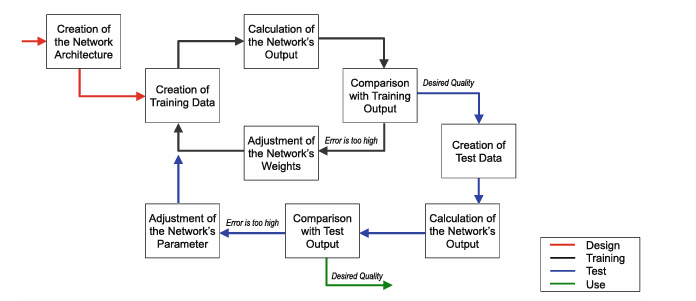
\includegraphics[width=1\textwidth]{Bilder/Training.png}
   \caption{Methodischer Ansatz zur Entwicklung neuronaler Netze \citep{lammel2012kunstliche}}
    \label{fig:training}
\end{figure}

\subsection{Promptbasierte Dialogsteuerung}
Im Kontext moderner KI-basierter Anwendungssysteme auf Basis generativer Sprachmodelle (Large Language Models) stellt das Prompt-Engineering eine zentrale Methode zur deterministischen Verhaltenssteuerung dar \citep{crocker2025softwareentwicklung}. Da autoregressive Sprachmodelle prinzipiell stochastisch operieren und Textausgaben auf Basis von Token-Wahrscheinlichkeiten generieren, dient die methodische Strukturierung der Eingabeanweisungen (Prompts) der Reduktion von Varianz und der Durchsetzung funktionaler, logischer oder tonaler Randbedingungen. In der computerlinguistischen Fachliteratur haben sich hierzu verschiedene fortgeschrittene Prompting-Techniken etabliert, die isoliert oder kombinatorisch eingesetzt werden, um die Kontrollierbarkeit und Zuverlässigkeit der Systemausgaben zu maximieren.

\subsubsection{Role Prompting}
Role Prompting basiert auf der expliziten Zuweisung einer spezifischen Systemidentität oder Rolle an das Sprachmodell innerhalb des System-Prompts \citep{zhang2023visar}. Mathematisch bewirkt diese Technik eine gezielte Konditionierung und Verengung des latenten Suchraums (Vektorraums) des Modells. Durch das Aktivieren von semantischen Clustern und Assoziationsketten, die mit der definierten Rolle korrespondieren, passt das Modell sowohl das Vokabular als auch das implizite Domänenwissen und die syntaktische Struktur der Zielausgabe an. Diese Form der Kontextualisierung verringert die Wahrscheinlichkeit von thematisch irrelevanten Ausgaben und stabilisiert die Tonalität des Dialogsystems über mehrere Interaktionsschritte hinweg.

\subsubsection{Structured Prompting}
Structured Prompting beschreibt die formale Strukturierung des Eingabetextes durch klar definierte Trennzeichen, XML/JSON-Tags oder Variablenplatzhalter \citep{hao2022structured}. Ziel dieser Technik ist es, eine eindeutige Trennung zwischen statischen Systeminstruktionen, dynamischen Kontextdaten und variablen Benutzerdatensätzen zu erzwingen. Durch die Verwendung strukturierter Masken kann ein übergeordnetes Softwaresystem externe, strukturierte Daten (z.\,B. aus Datenbanken oder algorithmischen Berechnungsebenen) zur Laufzeit dynamisch in den Prompt injizieren. Das Sprachmodell fungiert in dieser Architektur als rein ausführende generative Instanz, deren semantischer Handlungsrahmen durch die softwareseitig vorgegebenen Variablenwerte deterministisch limitiert wird.

\subsubsection{Chain-of-Thought Prompting}
Chain-of-Thought Prompting zwingt das Sprachmodell dazu, komplexe, mehrstufige Aufgabenstellungen nicht direkt zu beantworten, sondern den Transformationsprozess in eine Sequenz von logischen Zwischenschritten zu zerlegen \citep{wei2022chain}. Das Modell wird angewiesen, diesen inneren Monolog bzw. die logische Herleitung explizit zu verschriftlichen, bevor das finale Ausgabetoken generiert wird. Da LLMs Token für Token generieren, erlaubt die Erzeugung einer solchen intermediären Gedankenkette dem Modell, auf den zuvor selbst generierten logischen Zwischenschritten aufzubauen. Dies erhöht die mathematische und logische Präzision bei komplexen Schlussfolgerungsprozessen, schrittweisen Analysen oder der Einhaltung mehrstufiger, sequentieller Verhaltensregeln signifikant.

\subsubsection{Zero-Shot Prompting}
Zero-Shot Prompting beschreibt ein Verfahren, bei dem LLM eine spezifische Aufgabe ausschließlich über abstrakte Instruktionen, Regelwerke und Randbedingungen vorgegeben wird, ohne dass im Vorfeld exemplarische Eingabe-Ausgabe-Paare im Kontext hinterlegt werden \citep{brown2020language,ronanki2024requirements}. Diese Technik basiert auf der fundamentale Fähigkeit moderner, vortrainierter Transfomer-Modelle zur Generalisierung. Anstatt syntaktische Muster aus bereitgestellten Beispielen zu replizieren, dekonstruiert das Modell die abstrakte semantische Logik der Systemanweisungen und wendet sein im Pre-Training erworbenes, implizites Wissen direkt auf die neue Problemstellung an.


\section{Nutzung von KI-Chatbots im Coaching}
KI-basierte Chatbots haben in den letzten Jahren bereits vermehrt Einzug in den Coachingbereich gefunden. Sie werden zur Selbststeuerung von Personen oder Teams verwendet, um Entwicklungs- und Reflexionsprozesse zu unterstützen \citep{mai2020ai}. Coaching mit traumasensibler Ausrichtung verfolgt das Ziel, der Heilung durch Selbstregulation von Erregungszuständen und intensiven Emotionen \citep{Levine2010}. Daran anknüpfend wird eine Einordnung verschiedener Intensitäten von Belastungszuständen und psychische Belastungen herangezogen. 

Nach der NICE-Leitlinie wird zwischen milden, moderaten und schweren Störungen unterschieden \citep{kendrick2012common}. Ein milder Belastungszustand zeichnet sich durch wenig Symptome, eine begrenzte Dauer und geringe Auswirkungen auf den Alltag aus. Meist ist dies mit neu auftretenden Beschwerden oder mittelgradigen Problemen ohne Vorgeschichte verbunden. Von moderaten Belastungen spricht man, wenn eine deutliche Beeinträchtigung der Funktionalität vorliegt. Ein schwerer Belastungszustand liegt dann vor, wenn die Symptome eine erhebliche Beeinträchtigung der Funktionalität bewirken und über einen langen Zeitraum anhalten. Entsprechend ist eine intensivere Behandlung beziehungsweise Versorgung erforderlich, weshalb der Fokus dieser Arbeit auf dem Spektrum von milden bis moderaten Zuständen liegt.

\subsection{Related Work: Bisherige KI-basierte Erfolgsmodelle} \label{modell}
Im Folgenden werden zwei KI-basierte Erfolgsmodelle vorgestellt, die als Grundlage des in dieser Arbeit hergeleitete Chatbot-Modell dienen.

\subsubsection{MIND-SAFE Framework} 
Eine Referenzarchitektur für LLM-basierte Mental-Health-Chatbots ist das MIND-SAFE Framework, dessen Struktur in \ref{fig:mind} dargestellt ist. Ziel dieses Frameworks ist es, ein Dialogsystem bereitzustellen, dass therapeutisch fundiert arbeitet \citep{boit2025prompt}. Es werden ethische Standards beachtet und basiert auf einer personalisierten Struktur. Eine Kombination aus zugrundelegenden theoretischen Ansätzen und LLM Prompt Engineering führt zu einer mehrstufigen Sicherheitsarchitektur. Die erste Schicht ist der Input-Layer, der die Interaktion des Benutzers repräsentiert. Das bedeutet, der Nutzer gibt einen Text in den Chat ein, woraufhin eine Verarbeitung der Eingabe stattfindet. Es wird eine Risikoerkennung durchgeführt, um die spezifische Situation der Person zu erfassen, um vor allem gefährliche Inhalte frühzeitig zu erkennen. Die Dialog Ebene stellt den Kern des Systems dar und enthält drei zentrale Komponenten. In der User State Database wird der Zustand des Nutzers (zum Beispiel dessen Emotionen) im Zeitverlauf festgehalten, wodurch eine Personalisierung ermöglicht wird. Im zweiten Schritt erfolgt dann eine Retrieval-Argumented Generation. Das LLM greift auf eine Wissensbasis zu, die sich etablierten Therapieansätzen der kognitiven Verhaltenstherapie (CBT), Acceptance \& Commitment Therapy (ACT) oder Dialektisch-behaviorale Therapie (DBT) bedient. Dadurch wird ermöglicht, klinisch fundierte Antworten zu generieren. Der Promptengineering Layer strukturiert die therapeutische Gesprächsführung und steuert auf diese Weise Empathie, Tonalität und Interventionen. Durch das Multitier Safety System erfolgt eine mehrstufige Sicherheitsprüfung. Diese unterteilt sich in Pre-Generation Filter zur Risikoerkennung von LLM-Antworten, Post-Generation Filter zur Prüfung generierter Antworten und die Etical Guardrails, welche Regeln zur klinischen Sicherheit und zum Datenschutz beinhalten. Abschließend folgt ein kontinuierlicher Lernprozess. Dies meint eine Feedback-Schleife, wo Therapeuten und Experten die Nutzerinteraktionen prüfen und eine klinische Validierung und Verbesserung des Systems durchführen.

\begin{figure}[h!]
    \centering
    \includegraphics[width=1\textwidth]{Bilder/mind.png}
    \caption{Die Architektur des MIND-SAFE Frameworks \citep{boit2025prompt}}
    \label{fig:mind}
\end{figure}

\subsubsection{Digital Therapeutics (DTx) Komponentenmodell}
Die Grundidee des Frameworks ist ein Chatbot Modell, dass nicht nur aus einem Chatbot besteht, sondern mehrere funktionale Komponenten integriert \citep{baumel2025more}. Diese sind in \ref{fig:dtx} dargestellt. Damit soll eine höhere Wirksamkeit, Personalisierung und Skalierbarkeit therapeutischer Interventionen ermöglicht werden. Das Modell besteht aus fünf Kernkomponenten. Die Therapieeinheiten sind therapeutische Interventionen, wie Übungen oder Psychoedukation \citep{baumel2025more}. Psychoedukation verfolgt das Ziel, Klienten über eine Krankheit oder Behandlung zu informieren und damit ein Krankheitsverständnis, sowie den selbstverantwortlichen Umgang damit zu fördern \citep{bauml2018psychoedukation}.  Die KI kann an der Stelle Inhalte an Kontext oder Symptome der Klienten individuell anpassen. Die Entscheidungslogik bestimmt, wann und in welcher Reihenfolge Therapieeinheiten genutzt werden. Dies folgt dem Prinzip klassischer Entscheidungsbäume und schafft eine adaptive Anpassung an das Nutzerverhalten. Die narrative Ebene verbindet einzelnen Interventionen. Die Unterstützungsfunktion ergänzt menschliche Begleitung durch technische Hilfe. Das kann auch bedeuten, Feedback zum Verhalten zu geben oder den Nutzer zurück ins Programm zu holen. Die therapeutische Gesprächsinstanz ist die eigentlich zentrale dialogische Einheit des Systems. Die KI ermöglicht hier flexible und situationsspezifische Gespräche, Simulationen und Anpassung an Emotionen oder Zielsetzung des Prozesses. 

\begin{figure}[h!]
    \centering
    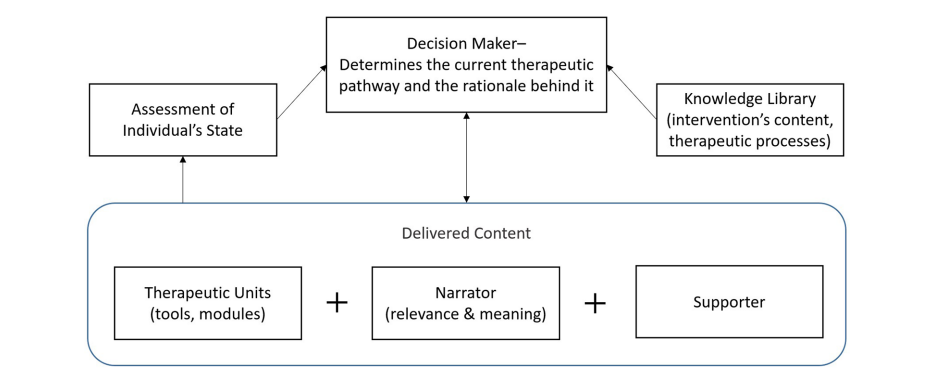
\includegraphics[width=1\textwidth]{Bilder/dtx.png}
    \caption{Die Komponenten der Digital Therapeutics \citep{baumel2025more}}
    \label{fig:dtx}
\end{figure}

\section{PSI-Theorie als psychologischer Bezugsrahmen}

Die Persönlichkeits-System-Interaktionen (PSI) Theorie nach \cite{Kuhl2000The} vereint Ansätze aus der Psychologie und Neurobiologie. Nach der PSI Theorie können kognitive und selbstregulatorische Mechanismen verändert werden. Dies wird durch die Art und Weise, wie eine Person Stimmungen und Gefühle, die sogenannten Affekte, reguliert, ermöglicht.
Die Theorie beleuchtet das menschliche Verhalten als Wechselspiel psychischer Systeme \citep{kuhl2005neue}. Es werden die vier Erkenntnissysteme Intentionsgedächnis, Intuitive Verhaltenssteuerung, Extentionsgedächnis sowie Objekterkennung unterschieden. Diese Systeme stehen in unmittelbarem Zusammenhang zueinander. Die Aktivierung der Systeme, sowie der Informationsaustausch zwischen diesen ist von den Affekten abhängig. Die Annahme der Theorie ist, dass unter Stress eine ängstliche oder traurige Stimmung vorherrscht, sodass der Mensch nicht mehr frei entscheiden kann, welches psychische System gerade aktiv ist. Bei positiver oder sicherer Stimmung hingegen besteht ein besseres Zusammenspiel der Systeme, was zur Selbstentwicklung beiträgt.


\subsection{Die vier psychischen Systeme}

\subsubsection{Intentionsgedächnis (IG)}
Das Intentionsgedächnis als analytisch sequentiell arbeitendes System ist zuständig für die Aufrechterhaltung von expliziten Absichten \citep{kuhl2005neue,kuhl2014psi}. Hier werden Ziele, Pläne und bewusste Entscheidungen gesteuert. Das IG wird besonders bei Hindernissen, Zielkonflikten oder fehlender Gelegenheit aktiv. Diese Aktivierung wird so lange aufrecht gehalten, bis eine Umsetzung des Ziels möglich ist. Dabei kommt es zur Hemmung, um vorschnelles Handeln zu vermeiden. Eine zu schwache Hemmung führt zu impulsivem Verhalten, eine zu starke kann Prokrastination, also das Aufschieben von Handlungen bewirken. Dies zeigt sich zum Beispiel, wenn man sich beim Vorhaben zu lernen ablenken lässt.

\subsubsection{Intuitive Verhaltenssteuerung (IVS)}
Die intuitive Verhaltenssteuerung ist einerseits bei der Umsetzung von Absichten und andererseits bei der Ausführung automatisierter Handlungsabläufe aktiv \citep{kuhl2014psi}. Im Gegensatz zum Intentionsgedächtnis arbeitet sie nicht primär bewusst und sequenziell, sondern verarbeitet Informationen parallel und unbewusst in Echtzeit. Dadurch ermöglicht sie ein spontanes, sensibles und situationangepasstes Verhalten, etwa in zwischenmenschlicher Kommunikation oder bei eingeübten Fertigkeiten, wie Auto fahren. Die IVS ergänzt das Intentionsgedächtnis, indem sie abstrakte Absichten in konkretes, an die jeweilige Situation angepasstes Handeln überführt.

\subsubsection{Extensionsgedächnis (EG)}
Das Extensionsgedächnis wird als (poly-)semantisches Netzwerk betrachtet, welches Aspekte wie Erfahrungen, Bedürfnisse und Werte der eigenen Person (des sogenannten Selbst) als ganzheitliches Wissen widerspiegelt \citep{kuhl2005neue,kuhl2014psi}. Dieses Wissen ist meist implizit und aus diesem Grund nicht immer vollumfänglich zugänglich. Es liefert eine Sammlung an persönlichen Lebenserfahrungen, die für die aktuelle Situation von Bedeutung sein könnten. Das EG ermöglicht die gleichzeitige
Berücksichtigung und Integration vieler Aspekte, die für komplexe Entscheidungen und gegenseitiges Verstehen von Menschen relevant sein können. Das Extensionsgedächnis und Selbst werden besonders durch persönliche Begegnungen aktiviert, bei denen gegenseitiges Verstehen eine zentrale Rolle spielt. Dies zeigt sich zum Beispiel in Partnerschaften oder auch der Verbindung zwischen Coach und Klient. Das EG kann Informationen und Gefühle simultan verarbeiten und integrieren, im Gegensatz zum analytisch-sequenziellen Denken des Intentionsgedächtnisses. Es ist für die Integration komplexer Erfahrungen relevant und ermöglicht insbesondere durch die Verarbeitung negativer Erlebnisse Selbstentwicklung und Lernsprünge. Dadurch zeigt sich wie bedeutend der Zugang des EG zur Selbstwahrnehmung für die Regulation von Gefühlen und damit auch die Verarbeitung negativer Erfahrungen ist.


\subsubsection{Objekterkennungssystem (OES)}
Das Objekterkennungssystem ermöglicht die bewusste Wahrnehmung einzelner, aus dem Gesamtkontext herausgelöster Aspekte und richtet die Aufmerksamkeit besonders auf Neuartiges, Fehler oder potenzielle Gefahren \citep{kuhl2005neue,kuhl2014psi}. Negative Stimmungen verstärken dabei den Fokus auf Unstimmigkeiten und Details, wie zum Beispiel das Versprechen während einer Präsentation. Das OES nimmt Einzelaspekte isoliert wahr, indem es sie aus dem Gesamtzusammenhang herauslöst. Das Extensionsgedächtnis integriert diese wieder in größere Zusammenhänge. Das Zusammenspiel beider Systeme ist wichtig für Lernen, Selbstentwicklung und situationsangemessenes Denken. Dabei hilft das OES beim Erkennen von Fehlern und Gefahren, das EG beim ganzheitlichen Verstehen und Einordnen von Erfahrungen.

\subsection{Modulationsannahmen der PSI-Theorie}
Die PSI-Theorie geht davon aus, dass positive und negative Affekte (Stimmungen und Gefühle) die Aktivierung und das Zusammenspiel der psychischen Systeme steuern \citep{kuhl2014psi}. Affekte beeinflussen die Aktivierung und Interaktionen der Systeme.  Gleichzeitig wirken die psychischen Systeme selbst wieder auf Affekte zurück. \cite{kuhl2014psi} beschreibt zwei zentrale Modulationsannahmen, die erklären, wie Affekte das Zusammenspiel der psychischen Systeme beeinflussen: 
\begin{enumerate}
  \renewcommand{\labelenumi}{(\arabic{enumi})}
  \item Willensbahnung: Die Umsetzung von Absichten durch die Zusammenarbeit von Intentionsgedächtnis (IG) und Intuitiver Verhaltenssteuerung (IVS)
  \item Selbstentwicklung durch Affektregulation: Selbstentwicklung durch die Interaktion von Objekterkennungssystem (OES) und Extensionsgedächtnis (EG)
\end{enumerate}

\subsubsection{Erste Modulationsannahme: Willensbahnung}
Die erste Modulationsannahme ist die Willensbahnung, die durch die Entstehung eines positiven Affekts und damit einem aktiven Intentionsgedächnisses entsteht \citep{Kuhl2000The}. Ein positiver Affekt erleichtert das Umsetzen von Intentionen, weil es eine höhere Bereitschaft zur Umsetzung gewährleistet. 

Das IG speichert Ziele und Absichten \citep{kuhl2005neue, kuhl2014psi}. Es wird besonders bei schwierigen oder unangenehmen Aufgaben aktiv und hält die Intention aufrecht. Herausforderungen reduzieren jedoch häufig den positiven Affekt, was dazu führen kann, dass die Umsetzung blockiert wird. Positive Affekte haben in diesem Zusammenhang eine entscheidende Rolle, weil sie das IVS aktivieren. Dadurch werden Hemmungen reduziert und flüssiges, spontanes Handeln ermöglicht. Statt die Absicht nur zu planen, kann eine tatsächliche Handlung entstehen. Positive Affekte, die dies ermöglichen, sind beispielsweise Motivation, Zuversicht, Ermutigung oder die Vorstellung eines erfolgreichen Ergebnisses.

\cite{kuhl2005neue} beschreibt die Fähigkeit der Frustrationstoleranz, wobei schwierige Absichten aufrechterhalten werden können, wenn negative Gefühle kurzfristig ausgehalten werden. Zur tatsächlichen Umsetzung von Absichten ist die Pendeltechnik geeignet. Diese basiert auf einem Wechsel von 1. der positiven Vorstellung des Zieles, 2. der bewussten Auseinandersetzung mit Schwierigkeiten und 3. der erneuten Aktivierung positiver Gefühle. Grundlage dessen ist ein flexibles Wechseln zwischen beiden Zustände.


\subsubsection{Zweite Modulationsannahme: Selbstentwicklung durch Affektregulation}
Die zweite Modulationsannahme beschreibt das Zusammenspiel von Objekterkennungssystem (OES) und Extensionsgedächtnis (EG) \citep{kuhl2005neue, kuhl2014psi}. Dabei wird das OES durch einen negativen Affekt aktiviert. Die Aufmerksamkeit richtet sich stärker auf Fehler, Unstimmigkeiten oder einzelne negative Aspekte, was dazu führt, dass der ganzheitliche Überblick verloren geht. Der Zugang zum Extensionsgedächtnis (EG) wird gehemmt, was zur Folge hat, dass negatives Denken die Wahrnehmung verengt und positive Erfahrungen oder alternative Sichtweisen weniger wahrgenommen werden. Auch der Zugang zu den eigenen Werten, Bedürfnissen oder Erfahrungen kann erschwert werden. Wenn der negative Affekt wieder reguliert wird, ist der Zugang zum EG erneut möglich, was Selbstwahrnehmung und die Integration von Erfahrungen fördert. Auf diese Weise ist Selbstreflexion, die Verarbeitung von Emotionen und damit eine Entwicklung möglich. Bei langanhaltenden negativen Affekten kann es passieren, dass fremde Ziele als eigene wahrgenommen werden und der Zugang zu den eigenen Bedürfnissen schwerfällt. Dies wird als Selbstfiltration bezeichnet und zeigt sich zum Beispiel, wenn eine Person die Erwartungen anderer übernimmt, ohne zu merken, dass diese nicht den eigenen Werten entspricht.

\begin{figure}[h!]
    \centering
    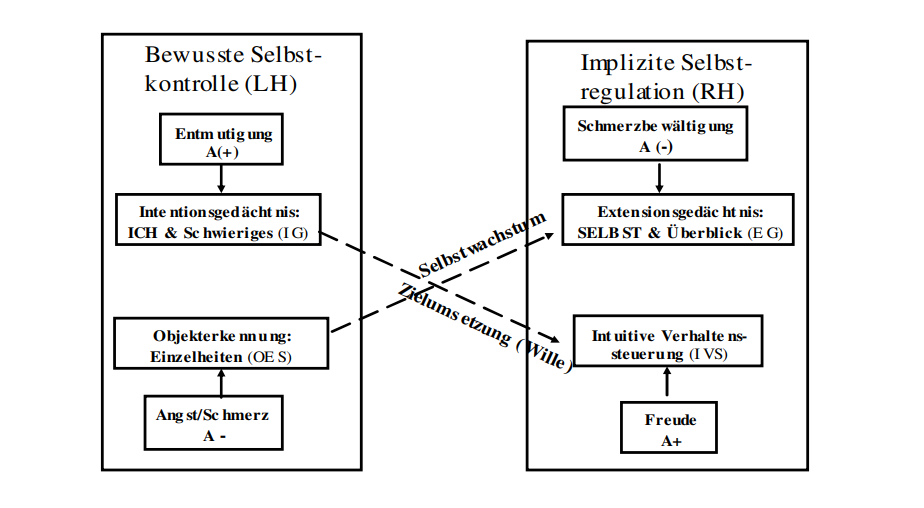
\includegraphics[width=1\textwidth]{Bilder/Modulationsannahmen.png}
    \caption{Schematische Darstellung der PSI-Theorie nach \cite{kuhl2005neue}}
    \label{fig:ma_kuhl}
\end{figure}

\subsubsection{Emotionale Steuerung von Verhalten}
Affektregulation wird als Grundlage von Willenskraft und Selbstentwicklung betrachtet und stellt somit eine zentrale Voraussetzung für die Selbststeuerung dar \citep{kuhl2005neue}. Das Zusammenspiel der einzelnen Systeme, Affekte und Modulationsannahmen sind in Abbildung \ref{fig:ma_kuhl} dargestellt. Selbstmotivierung entsteht durch die Regulation positiver Affekte und unterstützt somit die Umsetzung von Zielen. Selbstberuhigung ermöglicht die Verarbeitung belastender Erfahrungen, durch die Regulation von negativen Affekten. Der flexible Wechsel zwischen positiven und negativen Affekten wird als emotionale Dialektik bezeichnet. Weder dauerhaft positive noch dauerhaft negative Stimmung ist förderlich. Grundlage der Persönlichkeitsentwicklung ist die Fähigkeit, bewusster Selbstkontrolle und Gefühle situationsangemessen zu regulieren. Auf diese Weise fördern positive Affekte die Handlungsumsetzung (Willensbahnung), während negative Affekte helfen, Fehler und Probleme wahrzunehmen. Die anschließende Regulation negativer Gefühle ermöglicht Selbstreflexion und Lernen. 

Die Fähigkeit, Affekte eigenständig regulieren zu können, wird als Selbstkompetenz bezeichnet \citep{kuhl2014psi}. Dieser Lernprozess kann nur dann erfolgreich integriert werden, wenn die Beruhigung der Gefühle aus sich heraus bewältigt werden können, das heißt, wenn das „selbst“ in diesem Augenblick aktiv war. Eine positive Reaktion kann vor allem dann verknüpft werden, wenn Verständnis durch den Interaktionspartner gegeben ist. In der PSI-Theorie wird diese Verknüpfung der zwei Systeme, der affektiven Reaktion und des Selbst als Selbstkonditionierung bezeichnet.


\subsection{Bedeutung für Coachingprozesse} \label{prozess}
Die PSI-Theorie bietet eine gute Möglichkeit für Coachingprozesse, um Interventionen und Methoden abzuleiten \citep{kuhl2005neue}. Aus den Modulationsannahmen und damit der Integration der vier Systeme ergibt sich eine wichtige Implikation für Coachingprozesse. Demnach funktioniert Persönlichkeitsentwicklung umso besser, je besser die vier psychischen Systeme zusammenarbeiten. Selbstregulationsfähigkeiten entwickeln sich vor allem in Beziehungen. Gegenseitiges Verstehen gilt als zentrale Voraussetzung für Entwicklung. Auch emotionale Dialektik spielt im Coachingkontext eine elementare Rolle. Der Coach kann dem Klienten dabei helfen, Emotionen richtig Einzuordnen und sich nicht in emotionalen Zuständen zu verlieren, sondern Gefühle zu verarbeiten und für Motivation, sowie die Umsetzung einer Handlung zu nutzen. Zentrale Qualitäten vom Coaching sind im Kontext der PSI-Theorie, den Zugang zum Selbstsystem zu fördern, Selbstmotivierung zu stärken, Selbstberuhigung zu unterstützen, selbstkonguente Ziele zu entwickeln, emotionale Selbstregulation zu fördern und damit eine langfristige Selbststeuerung und Persönlichkeitsentwicklung zu ermöglichen. Coaching wirkt nicht primär durch Ratschläge, sondern durch eine zwischenmenschliche Beziehung.

\subsubsection{Schwerpunkt Selbstmotivierung (Erste Modulationsannahme)}
Die Pendeltechnik beschreibt den Wechsel zwischen positiven und negativen Affekten \citep{kuhl2005neue}. Es kann ein Perspektivwechsel zwischen Problembezogenheit und Ressourcenorientiertierung ermöglicht werden. Das Ziel besteht darin, nicht dauerhaft in einem negativen emotionalen Zustand zu verbleiben. Negative Gefühle werden also nicht einfach vermeiden oder unterdrückt, sondern die Fähigkeit zwischen emotionalen Zuständen flexibel wechseln können ermöglicht. Dadurch können belastende Erfahrungen wahrgenommen und verarbeitet werden. Gleichzeitig können positive, ressourcenorientierte Zustände zugänglich bleiben und emotionale Verarbeitung kann mit Motivation und Handlungsfähigkeit verbunden werden. Wenn der Fokus nicht ausschließlich auf Problemen oder Defiziten liegt, kann eine gezielte Aktivierung bereits vorhandener Ressourcen zu einem persönlichen Wachstum beitragen. Dadurch wird Zuversicht gefördert, Selbstwirksamkeit gestärkt, der Zugang zu positiven Erfahrungen ermöglicht und die Perspektive auf eigene Handlungsmöglichkeiten erweitert. Auf diese Weise wird wieder Verbindung zum EG, Selbstzugang, Integration und zur Handlungsaktivierung geschaffen. 

Die PSI-Theorie erklärt, dass Motivation und Zuversicht die Aufrechterhaltung von Absichten unterstützen können und das Vorstellen eines erfolgreichen Ergebnisses relevante psychische Systeme aktivieren können \citep{kuhl2005neue,kuhl2014psi}.

\subsubsection{Schwerpunkt Selbstberuhigung (Zweite Modulationsannahme)}
Unterstützung bei belastenden Erfahrungen und negativen Emotionen kann die Selbstberuhigung erleichtern \citep{kuhl2005neue, kuhl2014psi}. Der Coach kann den Klienten aus negativen Gedanken und Grübeln herausholen und stattdessen einen ganzheitlichen Blick auf die Situation liefern. Dies fördert die Integration neuer Erfahrungen in das Selbstsystem. Die Aktivierung des EG erfolgt besonders dann, wenn Menschen sich verstanden, gesehen und akzeptiert fühlen. Eine vertrauensvolle Beziehung, wie sie zwischen Coach und Klient gegeben sein sollte, kann den Zugang zu eigenen Ressourcen und Erfahrungen erleichtern und somit einen Rahmen schaffen, in dem diese eigenen Fähigkeiten gestärkt werden. 
Die Förderung der emotionalen und körperbezogenen Selbstwahrnehmung (des EG) kann an dieser Stelle eine Unterstützung darstellen \citep{storch2007ressourcenorientiertes}.

Ein Coach kann zum Beispiel bei der Regulation von Affekten eine Hilfe sein \citep{kuhl2014psi}. Die Verarbeitung negativer Erfahrungen gelingt nachhaltig vor allem dann, wenn sie emotional in das Selbstsystem integriert werden, statt lediglich kognitiv analysiert zu werden. Reines Reflektieren und argumentative Einordnung reichen dafür oft nicht aus, selbst wenn sie inhaltlich stimmig oder tröstlich erscheinen. 

Wiederholte positive Erfahrungen wie Trost, Ermutigung oder Verständnis fördern die Entwicklung der Selbstregulation, sodass langfristig positive emotionale Zustände selbstständig erzeugt werden können \citep{storch2007ressourcenorientiertes}. Wenn der Klient lernt, diese Funktionen schrittweise selbst zu übernehmen, kann emotionale Selbstständigkeit und Beziehungsfähigkeit gefördert werden. Unterstützung bei der Umsetzung schwieriger Ziele kann zur Selbstmotivierung beigetragen. Indem der Coach Interventionen zur Aktivierung persönlicher Ressourcen und Erfolgserfahrungen anleitet, kann der Klient einen besseren Zugang zum EG erlangen. Auf diese Weise kann die Entwicklung von Zuversicht gefördert werden. Durch die Regulation von Affekten kann eine Beruhigung belastender Gefühle zur Wiederherstellung eines Zustands führen, in dem weitere Verarbeitung möglich wird. Langfristig soll der Nutzer zunehmend zur Selbstberuhigung befähigt werden. Mögliche Schritte in diesem Kontext sind die Gefühle wahrnehmen und benennen und die Situation verlangsamen. Indem die Aufmerksamkeit auf regulierende und stabilisierende Aspekte gelenkt wird, Ressourcen aktiviert und Selbstberuhigung unterstützt wird. Interventionen sollen nicht ausschließlich auf kognitive Reflexion ausgerichtet sein. Auch die Wahrnehmung von Emotionen und Körperempfindungen spielt eine wichtige Rolle. Das Ziel besteht darin die Verbindung zwischen Körper, Emotion und persönlicher Bedeutung herzustellen. 
Durch die Reflexion von Werten und Bedürfnissen kann eine bewusste Unterscheidung zwischen den eigenen und fremden Erwartungen begünstigt werden. Ein Coachingziel kann somit die Vermeidung von Selbstinfiltration und Fremdbestimmung sein und damit auf die Entwicklung authentischer und persönlich passender Ziele ausgerichtet sein. Belastende oder neue Erfahrungen sollen nicht ausschließlich vermieden werden. Das Ziel ist eine Verarbeitung und Integration in den persönlichen Erfahrungskontext. Dadurch wird die Möglichkeit, aus Erfahrungen zu lernen und neue Handlungsmöglichkeiten zu entwickeln gespiegelt. Der Klient realisiert, wie er positiv mit Situationen umgeht und für sich selbst mehr Kapazität und Handlungsmöglichkeiten entwicklet. 


\subsection{Die sieben Systemebenen der PSI-Theorie}
Die PSI-Theorie betrachtet sieben Systemebenen, die menschliches Verhalten, bezüglich Umsetzung und Meidung der Motivation sowie entsprechende Affekte und Emotionen beschrieben \citep{kuhl2004systemdiagnostik, kuhl2014psi}. Im Kontext der Systemdiagnostik kann die Komplexität der Persönlichkeit im Gegensatz zu vielen klassischen Diagnostikansätzen detaillierter abgebildet werden. Klassische Persönlichkeitstests erfassen meist ausschließlich Persönlichkeitsmerkmale, sogenannte Erstreaktionen. Nach der Entwicklungsorientierten Osnabrücker Systemdiagnostik (EOS) wird außerdem betrachtet, wie eine Person mit Gedanken, Gefühlen und Problemen umgeht. Diese Selbstregulationsprozesse werden als Zweitreaktion bezeichnet. Anstatt Konstrukte wie „Selbstwirksamkeit“ oder „Persönlichkeit“ zu messen, betrachtet EOS über 100 Mikrofunktionskomponenten der Persönlichkeit, um konkrete Stärken und Entwicklungsfelder zu identifizieren. Coaching ist vor allem darauf ausgerichtet, wie eine Person Emotionen reguliert, mit Stress umgeht oder ihre Ressourcen aktiviert. Nach der EOS-Diagnostik wird ein zentraler Entwicklungshebel identifiziert, wodurch sich viele Verhaltensweisen erklären lassen. Coaching fokussiert sich demnach auf individuelle statt standardisierte Interventionen sowie emotionale Selbstregulation. Negative Emotionen werden nicht als Problem betrachtet, sondern als wichtige Information über Konflikte und Bedürfnisse. Diese Betrachtung steht in direktem Zusammenhang zur zweiten Modulationsannahme der PSI-Theorie.

Dieser Ansatz ist von besonderer Relevanz für Coachings, vor allem auch im traumasensiblen Arbeiten. Traumaheilung entsteht durch die Fähigkeit, Erregungszustände selbst zu regulieren und intensive Emotionen halten und verarbeiten zu können \citep{Levine2010}. EOS und Traumaarbeit fokussieren eine Prozess- statt Defizitorientierung, sowie die Ausrichtung auf selbstregulatorische Prozesse.

Darauf basierend werden sieben Quellen der menschlichen Motivation abgeleitet, die einen Leitfaden für Coachings liefern, um unter Betrachtung der Erst- und Zweitreaktion erfolgreiche Interventionen und Konzepte abzuleiten \citep{kuhl2004systemdiagnostik, kuhl2014psi}. 

\subparagraph{1) Automatisches Verhalten und Erkennen}
Diese Ebene umfasst gelernte Routinen und automatische Handlungen. Verhalten oder eine Reaktion wird automatisch durch einen entstehenden Reiz ausgelöst und braucht somit keine bewusste Steuerung. Wenn keine förderlichen Gewohnheiten existieren, bestehen Schwierigkeiten beim Aufbringen von Motivation.

\subparagraph{2) Temperament}
Temperament stellt die grundsätzliche Erregbarkeit und Aktivierung einer Person dar. Das bedeutet, wie stark wird auf einen Reiz reagiert und wie ist die generelle Handlungsenergie. Eine zu geringe Aktivierung kann zur Antriebslosigkeit führen, während eine besonders hohe Aktivierung zu Unruhe und Impulsivität führt.

\subparagraph{3) Affekte und Anreize}
Die dritte Ebene beschreibt die emotionale Bewertung von Erfahrungen. Auf der einen Seite stehen positive Affekte wie Freude oder Belohnung und demgegenüber negative Affekte, wie Angst, Ärger oder Stress. Motivation entsteht demnach durch eine Verknüpfung von Objekten mit Emotionen. Fehlende Motivation zum Lernen besteht zum Beispiel, wenn das Lernen negativ assoziiert ist.

\subparagraph{4) Stressbewältigung}
Bei der Stressbewältigung geht es darum, ob unter Stress eine höhere Steuerung erhalten bleibt. Progression bedeutet, dass eigene Ziele und Selbststeuerung aktiv bleiben. Regression andererseits meint einen Rückfall in impulsives Verhalte, Affekte oder Gewohnheiten. Unter Stress kann somit das Reaktionsvermögen verloren gehen.

\subparagraph{5) Motive: Kraftquellen}
Motive sind unbewusste Bedürfnisse wie beispielsweise Anerkennung, Macht, Beziehung oder Autonomie. Sie wirken oft implizit und steuern eine langfristige Zielausrichtung. Werden diese Ziele und Bedürfnisse angesprochen, kann das intrinsische Motivation, wenn auch unbewusst, erhöhen.

\subparagraph{6) Denken und Fühlen}
Als kognitive Ebene werden bewusste Gedanken, konkrete Ziele und Bedeutungsstrukturen betrachtet. Das eigene Selbstbild und Sinnzuschreibungen spielen in diesem Kontext eine Rolle zur Motivation, in dem sie Orientierung und Identifikation liefern.

\subparagraph{7) Selbststeuerung}
Die Selbststeuerung wird als höchste Ebene verstanden. Sie koordiniert das Zusammenwirken der einzelnen Systeme Selbstkontrolle, Selbstregulation, Selbstmotivierung und das Lernen aus Erfahrungen. \citep{ritz2008personlichkeitsorientierte, kuhlsieben}


\section{Systematische Literaturübersicht}
Die Vorgehensweise der Literaturrecherche folgt dem systematischen Aufbau nach \cite{webster2002analyzing}. Für die Stichwortsuche wurden die Literaturdatenbanken Google Scholar, ScienceDirect, Ieeeexplore und Scopus herangezogen. Faktoren wie Zitationen des gefundenen Artikels und 
Reputation der Autoren wurden verwendet, um einzuschätzen, ob es sich um eine hochwertige wissenschaftliche Quelle handelt. Es wurden Suchwörter wie \glqq Chatbot and Coaching\grqq{} or \glqq PSI and Coaching\grqq{} or \glqq LLM and Coaching\grqq{} eingegeben, um passende Literatur zu finden. Im zweiten Schritt folgte eine Rückwärtssuche, in der anhand der Referenzen der gefundenen Artikel aus dem ersten Schritt weitere relevante Artikel überprüft und in die Suche miteinbezogen wurden. 
Mit der daraus resultierenden Sammlung an 
Artikeln und Büchern wurde im letzten Schritt eine Vorwärtssuche durchgeführt und es entstand ein Pool an 
relevanten Artikeln. Zuletzt folgte eine intensive Auseinandersetzung mit iterativer Aussortierung der 
nicht-relevanten Artikel und Beiträge, die thematisch nicht zur Forschungsfrage passen.

\subsection{Forschungslücke}

Obwohl sich KI-gestützte Chatbots im Coaching- und therapeutischen Sektor zunehmend als digitale Selbstcoaching-Tools etablieren \citep{mai2023chatbots} und erste klinisch fundierte Referenzarchitekturen wie das MIND-SAFE Framework existieren \citep{boit2025prompt}, offenbart die systematische Literaturanalyse Forschungslücken an der Schnittstelle zwischen Wirtschaftsinformatik, dialogischer KI und psychologischer Systemtheorie.

Eine Forschungslücke ergibt sich aus der fehlenden informationstechnischen Modellierung der PSI-Theorie. Bestehende Mental-Health-Anwendungen stützen sich vorwiegend auf die algorithmische Abbildung klassischer, strukturell linearer Ansätze wie der kognitiven Verhaltenstherapie (CBT) oder der Dialektisch-behavioralen Therapie (DBT) \citep{boit2025prompt}. Es fehlt jedoch an einer operationalisierten Entscheidungs- und Dialogsteuerungslogik, die auf ganzheitlichen, neurobiologisch fundierten Persönlichkeits-System-Interaktionen (PSI) basiert \citep{Kuhl2000The}. Die computerlinguistische Modellierung des dynamischen Zusammenspiels zwischen den vier Makrosystemen (IG, IVS, EG, OES) und deren affektiver Modulation ist in der aktuellen Literatur nicht vorhanden.
    
Ein zweiter Kernpunkt stellen aktuelle Forschungsansätze im Bereich der Personalisierung des LLM dar. Diese fokussieren sich primär darauf, Interaktionen und Inhalte an die individuellen Nutzerpräferenzen anzupassen \citep{Tan2024}. Im traumasensiblen Coaching birgt diese rein reaktive Anpassung jedoch das Risiko, dass das generative Sprachmodell nicht-entwicklungsfördernden Verhaltens- und Denkmuster des Klienten adaptiert, spiegelt und somit unbewusst verfestigt \citep{Xiao2025Humanizing}. Es existiert eine Forschungslücke hinsichtlich der Frage, wie dialogische KI durch proaktive, theoriegeleitete Impulse so gestaltet werden kann, dass sie diese traumabedingten Schutzstrategien sichtbar macht, aktiv hinterfragt und transformiert, anstatt sie lediglich stochastisch zu reproduzieren.

Des Weiteren wurde ein Mangel an deterministischen Design- und Interaktionsmerkmalen für traumasensible LLMs herausgestellt. Die Arbeit knüpft an dieser Stelle an und zeigt eine präzise funktionale Ausgestaltung von Prompts, die sowohl diagnostisch als auch affektregulierend wirken \citep{kuhl2004systemdiagnostik, Levine2010}. Bisher stellt dies im Kontext von Personen mit leichten bis moderaten psychischen Belastungen eine Lücke der Forschung dar.

Während die technische Machbarkeit von dialogischer KI weit fortgeschritten ist, fehlt es an der theoretisch-konzeptionellen Ausarbeitung, die psychologische Wirkmechanismen der Affektregulation und Selbststeuerung in eine deterministische Systemarchitektur überführen. Diese Lücke wird durch das in dieser Arbeit entwickelte PSI-basierte Coaching-Modell adressiert.
